\documentclass{../harvardml}

% Authors: 
% Edited by: Mark Goldstein + others (jan 2018)
% Edited by: Amir Shanehsazzadeh, Andrew Kim, Nari Johnson (Jan 2021)
% Edited by: Max Guo, Raphael Pellegrin, Katherine Tian (Jan 2022)
% Edited once more by: William Tong (Jan 2023) + Skyler Wu (Jan 2023)
% Edited once more by: Jeffrey Xu (Jan 2024) + Gabriel Sun (Jan 2024)
% Edited once more by: Gabriel Sun (Jan 2025)

% Adapted from CS281 Fall 2019 section 0 notes

% This tex file relies on
% the presence of two files:
% harvardml.cls and common.sty

\course{CS1810-s25}
\assignment{Homework \#0}
\duedate{January 31, 2025 at 11:59 PM}

\usepackage{url}
\usepackage{float}
\usepackage{amsfonts, amsmath, amsthm}
\usepackage{listings}
\usepackage[shortlabels]{enumitem}
\usepackage{hyperref}
\usepackage{etoolbox}
\usepackage{bm}

\theoremstyle{definition}
\newtheorem{defn}{Definition}[section]
\theoremstyle{plain}
\usepackage[textsize=tiny]{todonotes}
\usepackage{../common}


%%%%%%%%%%%%%%%%%%%%%%%%%%%%%%%%%%
%% Solution environment
\usepackage{xcolor}
\usepackage{comment}
\newenvironment{solution}
  {\color{blue}\section*{Solution}}
{}
%%%%%%%%%%%%%%%%%%%%%%%%%%%%%%%%%%


\begin{document}



\noindent Welcome to CS1810! The purpose of this assignment is to help assess your readiness for this course.  It will be graded for completeness and effort.  \textbf{Areas of this assignment that are difficult are an indication of areas in which \emph{you} need to self-study. If you find you are struggling with many of these questions, it might be prudent to postpone taking this course until after you have mastered the necessary prerequisites.  \emph{During the term, the staff will be prioritizing support for new material taught in CS1810 over teaching prerequisites.}  If you are unsure about your readiness, please contact the head TFs for advice.}


\begin{enumerate}
    \item Please type your solutions after the corresponding problems using this \LaTeX\ template, and start each problem on a new page.
    \item Please submit the \textbf{writeup PDF to the Gradescope assignment `HW0'}. Remember to assign pages for each question.
    \item Please submit your \textbf{\LaTeX\ file and code files (i.e., anything ending in \texttt{.py}, \texttt{.ipynb}, or \texttt{.tex}) to the Gradescope assignment `HW0 - Supplemental'}. 
\end{enumerate}

\newpage
\begin{problem}[Modeling Linear Trends - Linear Algebra Review]
In this class, we will be exploring the question of ``how do we model the trend in a dataset" under different guises. In this problem, we will explore the algebra of modeling a linear trend in data. We call the process of finding a model that capture the trend in the data, ``fitting the model."\\

\noindent \textbf{Learning Goals:} In this problem, you will practice translating machine learning goals (``modeling trends in data") into mathematical formalism using linear algebra. You will explore how the right mathematical formalization can help us express our modeling ideas unambiguously and provide ways for us to analyze different pathways to meeting our machine learning goals.\\

\noindent Let's consider a dataset consisting of two points $\mathcal{D} = \{(x_1, y_1), (x_2, y_2)\}$, where $x_n, y_n$ are scalars for $n=1, 2$. Recall that the equation of a line in 2-dimensions can be written: $y = w_0 + w_1x$. 
\begin{enumerate}
    \item Write a system of linear equations determining the coefficients $w_0, w_1$ of the line passing through the points in our dataset $\mathcal{D}$ and analytically solve for $w_0, w_1$ by solving this system of linear equations (i.e., using substitution). Please show your work.
    \item Write the above system of linear equations in matrix notation, so that you have a matrix equation of the form $\mathbf{y} = \mathbf{X}\mathbf{w}$, where $\mathbf{y}, \mathbf{w} \in \mathbb{R}^2$ and $\mathbf{X} \in \mathbb{R}^{2\times 2}$. For full credit, it suffices to write out what $\mathbf{X}$, $\mathbf{y}$, and $\mathbf{w}$ should look like in terms of $x_1$, $x_2$, $y_1$, $y_2$, $w_0$, $w_1$, and any other necessary constants. Please show your reasoning and supporting intermediate steps.
    \item Using properties of matrices, characterize exactly when an unique solution for  $\mathbf{w}=\left(w_0 \; w_1 \right)^{T}$ exists. In other words, what must be true about your dataset in order for there to be a unique solution for $\mathbf{w}$? When the solution for $\mathbf{w}$ exists (and is unique), write out, as a matrix expression, its analytical form (i.e., write $\mathbf{w}$ in terms of $\mathbf{X}$ and $\mathbf{y}$).
    
    Hint: What special property must our $\mathbf{X}$ matrix possess? What must be true about our data points in $\mathcal{D}$ for this special property to hold?
    \item Compute $\mathbf{w}$ by hand via your matrix expression in (3) and compare it with your solution in (1). Do your final answers match? What is one advantage for phrasing the problem of fitting the model in terms of matrix notation? 
    \item In real-life, we often work with datasets that consist of hundreds, if not millions, of points. In such cases, does our analytical expression for $\mathbf{w}$ that we derived in (3) apply immediately to the case when $\mathcal{D}$ consists of more than two points? Why or why not?

\end{enumerate}
    
\end{problem}

\newpage


\begin{solution}


    \subsection*{1.1 Linear Equation}
    Given the equation of a line:
    
    \begin{equation}
        y = w_0 + w_1 x
    \end{equation}
    
    Using the given points:
    
    \[
    \begin{cases}
        w_0 + w_1 x_1 = y_1 \\
        w_0 + w_1 x_2 = y_2
    \end{cases}
    \]
    
    From equation (1):
    
    \begin{equation}
        w_1 = \frac{y_2 - y_1}{x_2 - x_1}
    \end{equation}
    
    Using equation (2):
    
    \begin{equation}
        w_0 = y_2 - w_1 x_2
    \end{equation}
    
    Substituting $w_1$:
    
    \begin{equation}
        w_0 = y_2 - \left(\frac{y_2 - y_1}{x_2 - x_1} \right) x_2
    \end{equation}
    
    Thus, the final expressions for $w_1$ and $w_0$ are:
    
    \[
    w_1 = \frac{y_2 - y_1}{x_2 - x_1}
    \]
    
    \[
    w_0 = y_2 - \left(\frac{y_2 - y_1}{x_2 - x_1} \right) x_2
    \]
    
    \subsection*{1.2 Matrix Notation}
    
    We represent the equations in matrix form:
    
    \[
    \bm{y} = \bm{X} \bm{w}
    \]
    
    \[
    \begin{bmatrix}
        y_1 \\
        y_2
    \end{bmatrix}
    =
    \begin{bmatrix}
        1 & x_1 \\
        1 & x_2
    \end{bmatrix}
    \begin{bmatrix}
        w_0 \\
        w_1
    \end{bmatrix}
    \]
    
    We include the column of ones to ensure that the intercept term is included.

    \subsection*{1.3 Unique Solution Conditions}
        For there to be a unique solution $\bm{w}$, we need $\bm{X}$ to be a linearly independent matrix -- the rows of $\bm{X}$ should be linearly independent of each other. In this case, we require:

        \begin{equation}
            \det(\bm{X}) \neq 0
        \end{equation}

        Thus:
        \begin{equation}
            \det(\bm{X}) = \begin{vmatrix}
                1 & x_1 \\
                1 & x_2
            \end{vmatrix} = x_2 - x_1 \neq 0
        \end{equation}

        Therefore:
        \[
        x_2 - x_1 \neq 0
        \]

        This condition ensures there is no duplicate solution, as having $x_2 = x_1$ would lead to a non-unique solution.

            
    \subsection*{1.4 Solution Using Gaussian Elimination}
    
    The system:
    
    \[
    \begin{bmatrix}
        1 & x_1 \\
        1 & x_2
    \end{bmatrix}
    \begin{bmatrix}
        w_0 \\
        w_1
    \end{bmatrix}
    =
    \begin{bmatrix}
        y_1 \\
        y_2
    \end{bmatrix}
    \]
    
    Using Gaussian elimination:
    
    \[
    \begin{bmatrix}
        1 & x_1 & y_1 \\
        1 & x_2 & y_2
    \end{bmatrix}
    \]
    
    Subtracting row 1 from row 2:
    
    \[
    \begin{bmatrix}
        1 & x_1 & y_1 \\
        0 & x_2 - x_1 & y_2 - y_1
    \end{bmatrix}
    \]
    
    Solving for $w_1$:
    
    \[
    w_1 = \frac{y_2 - y_1}{x_2 - x_1}
    \]
    
    Substituting in the first equation:
    
    \[
    w_0 = y_1 - w_1 x_1
    \]
    
    Thus, we get the same result as before.
    
    \subsection*{1.5 Higher Dimensions}
    
    If we have more than two points, we need to extend our equations. Changes in dimensions:
    
    \begin{itemize}
        \item $\bm{y}$ becomes an $n \times 1$ vector.
        \item $\bm{X}$ becomes an $n \times 2$ matrix.
        \item $\bm{w}$ remains a $2 \times 1$ vector.
    \end{itemize}
    
    In general, if all points do not lie on the same line, there may be no exact solution, requiring methods such as least squares regression.
    


    
\end{solution}

\color{black}
\newpage


\begin{problem}[Optimizing Objectives - Calculus Review]
In this class, we will write real-life goals we want our model to achieve into a mathematical expression and then find the optimal settings of the model that achieves these goals. The formal framework we will employ is that of mathematical optimization. Although the mathematics of optimization can be quite complex and deep, we have all encountered basic optimization problems in our first calculus class!\\

\noindent \textbf{Learning Goals:} In this problem, we will explore how to formalize real-life goals as mathematical optimization problems. We will also investigate under what conditions these optimization problems have solutions.\\

\noindent In her most recent work-from-home shopping spree, Nari decided to buy several house plants. \textit{Her goal is to make them to grow as tall as possible.} After perusing the internet, Nari learns that the height $y$ in mm of her Weeping Fig plant can be directly modeled as a function of the oz of water $x$ she gives it each week:
$$y = - 3x^2 + 72x + 70.$$
\begin{enumerate}
    \item First, plot the height function. What does the plot tell you about the existence and uniqueness of a maximum plant height? Next, support your claim solely based on the form of the function.

    \item Use calculus to find how many ounces of water per week Nari should give to her plant in order to maximize its height. With this much water, how tall will her plant grow?

\end{enumerate}
Now suppose that Nari want to optimize both the amount of water $x_1$ (in oz) \textit{and} the amount of direct sunlight $x_2$ (in hours) to provide for her plants. After extensive research, she decided that the height $y$ (in mm) of her plants can be modeled as a two variable function:

$$y = f(x_1, x_2) = \exp\left(-(x_1 - 2)^2 - (x_2 - 1)^2 \right)$$
\begin{enumerate}
    \setcounter{enumi}{2}
    \item Using \texttt{matplotlib}, visualize in 3D the height function as a function of $x_1$ and $x_2$ using the \texttt{plot\_surface} utility for $(x_1, x_2) \in (0, 6) \times (0, 6)$. Then, determine the values of $x_1$ and $x_2$ that maximize plant height. Do these yield a global maximum? 
    
    Hint: You don't need to take any derivatives here; reasoning about the form of $f(x_1, x_2)$ suffices.
\end{enumerate}
\end{problem}

\newpage


\begin{solution}
	
\subsection*{2.1}
The plot tells us that there is exactly \textbf{one maximum} and \textbf{no minimum}. \\
This is because the curve is concave down at all points, as shown by:

\[
\frac{d^2y}{dx^2} = -6
\]

\begin{center}
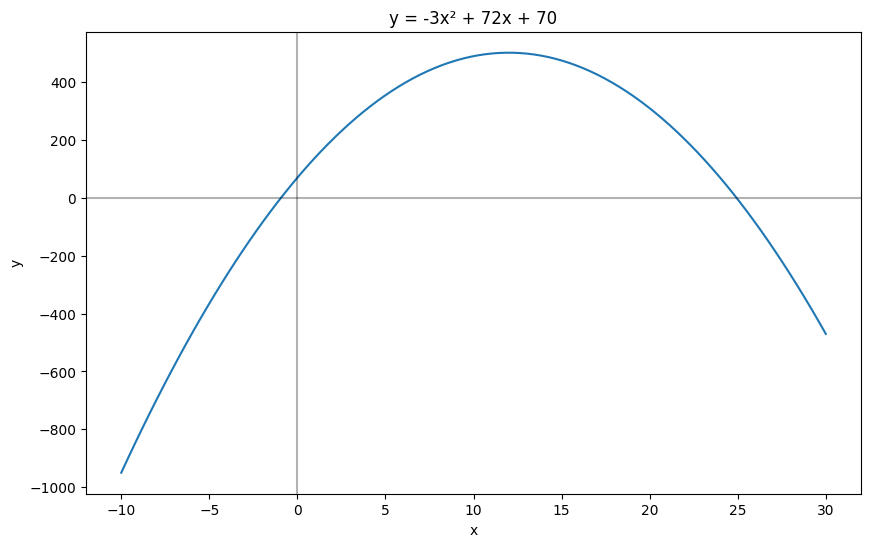
\includegraphics[width=0.5\textwidth]{images/2.1.png}
\end{center}

\subsection*{2.2}
Given:

\[
\frac{dy}{dx} = -6x + 72
\]

Setting the first derivative to zero to find critical points:

\[
0 = -6x + 72
\]

\[
72 = 6x
\]

\[
x = 12
\]

Since the second derivative is negative:

\[
\frac{d^2y}{dx^2} = -6
\]

This confirms that the function is concave down, meaning we have found a \textbf{maximum} at:

\[
x_c = 12
\]

The function value at this point is:

\[
-3(12)^2 + 72(12) + 78
\]

\[
= -3(144) + 864 + 78
\]

\[
= -432 + 864 + 78
\]

\[
= 510
\]

Thus, the maximum value is:

\[
\mathbf{510} \text{ inches}
\]

\subsection*{2.3}
Yes, this yields a maximum. \\

As \( x \) increases from a small value, the height increases. \\

As \( x \) further increases, the height begins to decrease, reaching smaller and smaller values beyond the peak. \\

Since the height never exceeds this maximum again, \textbf{this is a global maximum}.

\end{solution}


\begin{center}
    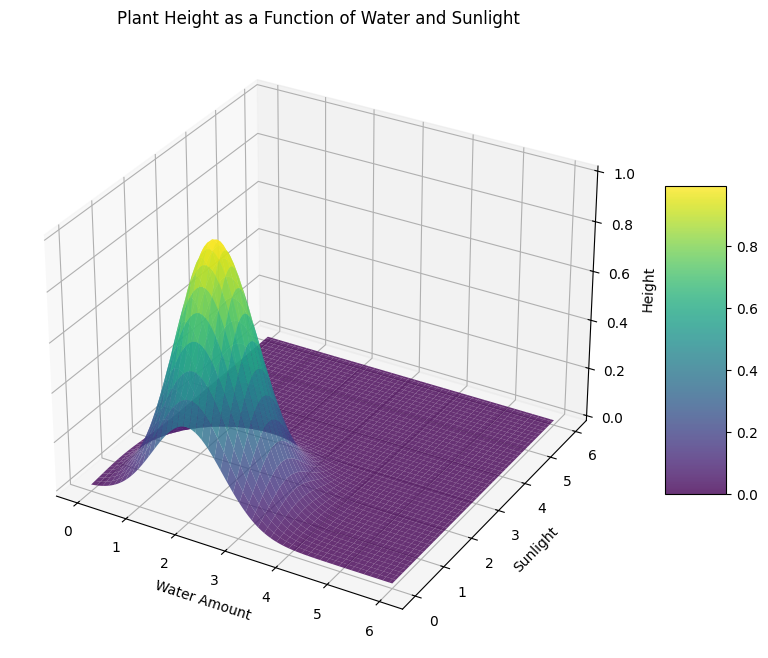
\includegraphics[width=0.5\textwidth]{images/2.3.png}
    \end{center}

\newpage 


\begin{problem}[Reasoning about Randomness - Probability and Statistics Review]
In this class, one of our main focuses is to model the unexpected variations in real-life phenomena using the formalism of random variables. In this problem, we will use random variables to model how much time it takes an USPS package processing system to process packages that arrive in a day.\\

\noindent \textbf{Learning Goals:} In this problem, you will analyze random variables and their distributions both analytically and computationally. You will also practice drawing connections between said analytical and computational conclusions.\\

\noindent Consider the following model for each package that arrives at the US Postal Service (USPS):
\begin{itemize}
    \item Every package has a random size $S$ (measured in $in^3$) and weight $W$ (measured in pounds), with joint distribution
    $$(S, W)^{T} \sim \mathcal{N}\left( \boldsymbol{\mu}, \boldsymbol{\Sigma}\right) \text{, with } \boldsymbol{\mu} = \begin{bmatrix} 120 \\ 4 \end{bmatrix} \text{ and } \boldsymbol{\Sigma} = \begin{bmatrix} 1.5 & 1 \\ 1 & 1.5 \end{bmatrix}.$$ 
    \item The size and weight of each package is independent of those of all the other packages.
    \item Processing time $T$ (in seconds) for each package is given by $T = 60 + 0.6 W + 0.2 S + \epsilon$, where $\epsilon$ is an independent random noise variable with Gaussian distribution $\epsilon \sim \mathcal{N}(0, 5)$.
\end{itemize}

\begin{enumerate}
    \item Perform the following tasks:
    \begin{enumerate}
        \item Give one reason for why the Gaussian distribution may not be appropriate for modeling the size and weight of packages.
        
        \item Empirically estimate the most likely combination of size and weight of a package by sampling 500 times from the joint distribution of $S$ and $W$ and generating a bivariate histogram of your $S$ and $W$ samples. A visual inspection is sufficient -- you do not need to be incredibly precise.  How close are these empirical values to the theoretical expected size and expected weight of a package, according to the given Bivariate Gaussian distribution?

        Hint: For this part, you may find the \texttt{multivariate\_normal} module from \texttt{scipy.stats} especially helpful. You may also find the \texttt{seaborn.histplot} function quite helpful. 
    \end{enumerate}
    
    \item For 1001 evenly-spaced values of $W$ between $0$ and $10$, plot $W$ versus the joint Bivariate Gaussian PDF $p(W, S)$ with $S$ fixed at $S=118$. Repeat this procedure for $S$ fixed at $S=122$. Comparing these two PDF plots, what can you say about the correlation of random variables $S$ and $W$? 
    
    \item Because $T$ is a linear combination of random variables, it itself is a random variable. Using properties of expectations and variance, please compute $\mathbb{E}(T)$ and $\mathrm{Var}(T)$ analytically.
    
    \item Define $N$ to be the number of packages that arrive today, and suppose that packages that weigh less than 4 pounds are considered fragile. Conditional on $N=n$, what is the name and PMF of the distribution of the number of fragile packages that arrive today?
    
    \item Now suppose that $N = \sum_{h=1}^{24}P_h$, where the $P_h$ are independent and identically distributed as $\text{Pois}(\lambda=3)$. Then define $T^* = \sum_{i=1}^{N} T_i$ as the  \textit{total} amount of time it takes to process \textit{all} these packages, where $T_i$ follows the distribution of $T$ that we previously defined for each package.
    \begin{enumerate}
        \item Write a function to simulate draws from the distribution of $T^{*}$. 
        \item Using your function, empirically estimate the mean and standard deviation of $T^{*}$ by generating $1000$ samples from the distribution of $T^{*}$.
    \end{enumerate}

\end{enumerate}
\end{problem}



\newpage

\begin{solution}
	\section*{3.1}

\subsection*{(a)}
Both \textbf{size} and \textbf{weight} cannot be negative, but the Gaussian distribution contains negative values.

(b)
\begin{center}
    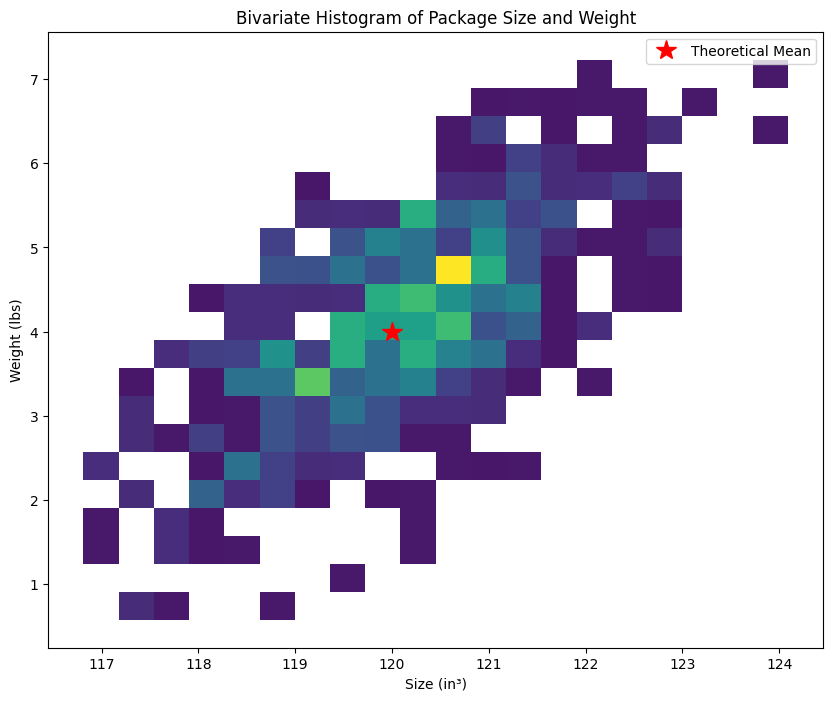
\includegraphics[width=0.5\textwidth]{images/3.1.png}
    \end{center}

\section*{3.2}

\begin{center}
    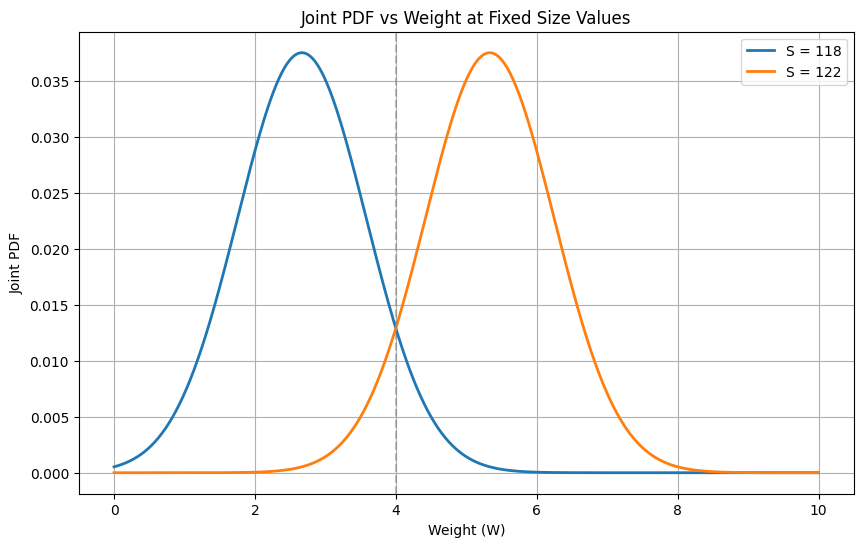
\includegraphics[width=0.5\textwidth]{images/3.2.png}
    \end{center}


\section*{3.3}
We start with the expectation equation:

\[
E[T_J] = 60 + 0.6E[W] + 0.2E[S] + E[\epsilon]
\]

Given:
\[
E[W] = 4, \quad E[S] = 120, \quad E[\epsilon] = 0
\]

Substituting the values:

\[
E[T_J] = 60 + 2.4 + 24 + 0
\]

\[
\boxed{E[T_J] = 86.4}
\]

Next, we compute the variance:

\[
\text{Var}[T_J] = \text{Var}[60 + 0.6W + 0.2S + \epsilon]
\]

Since variance is \textbf{location invariant}, we simplify:

\[
= \text{Var}[0.6W + 0.2S + \epsilon]
\]

Given that the covariances are not zero, \( S \) and \( W \) are not independent. Hence:

\[
\text{Var}[0.6W + 0.2S] + \text{Var}[\epsilon]
\]

Expanding:

\[
= \text{Var}[0.6W] + \text{Var}[0.2S] + 2\text{Cov}(W, S) + 5
\]

Given values:

\[
\text{Var}[W] = 1.5, \quad \text{Var}[S] = 1.5, \quad \text{Cov}(W, S) = 1
\]

\[
= (0.6^2 \times 1.5) + (0.2^2 \times 1.5) + (2 \times 0.6 \times 0.2 \times 1) + 5
\]

\[
= (0.36 \times 1.5) + (0.04 \times 1.5) + (2 \times 0.6 \times 0.2 \times 1) + 5
\]

\[
= 0.54 + 0.06 + 0.24 + 5
\]

\[
= 7.6
\]

\[
\boxed{\text{Var}[T_J] = 7.6}
\]

\section*{3.4}
This follows the \textbf{binomial distribution}:

\[
\text{Bin}(p, n)
\]

- There is a set number of trials.
- There is a set probability of a package being considered feasible.
- We are interested in the count of those.

\end{solution} 

\newpage 

\begin{problem} [Implementing a Linear Regression - Coding Review]
In this class, we will bridge theory and practice through implementing the methods that we cover from scratch. In this problem, we follow up on Problem 1 through exploring a more practical version of linear regression (fitting a linear model). Namely, we use ordinary least squares (OLS) to estimate a \textit{line of best fit} rather than a perfect fit to our data. Note that the focus of this problem is on coding rather than math---we will cover the relevant theory in much more depth during the course.\\

\noindent \textbf{Learning Goals:} In this problem, you will gain experience with the procedure of modeling real-world data. You will also get useful practice with debugging and writing clean, efficient code in Python. \\

\noindent Steve is a fictional CS 1810 TF giving a live demo of how to fit a linear regression. However, he quickly realizes that coding live in front of an audience isn't for the faint of heart. As a star student, you will help him with his code. Just like Problem 1, the demo uses a 2-D dataset, so that the goal is to model the relationship between the $x$ and $y$ coordinates. The data are stored in the \texttt{data} variable, with the first column corresponding to the $x$-coordinate and the second corresponding to the $y$-coordinate. 

\begin{enumerate}
    \item Using the provided data, Steve has defined variables $\texttt{y}$ and $\texttt{x}$ corresponding to the respective coordinates.  What is wrong with his current code? Fix the code and then plot the data. Does there appear to be a linear trend?

    \item Steve then defines a new variable \texttt{X}, which is meant to resemble $\bm X$ from Problem 1. Specifically, \texttt{X} is supposed to have one column of all ones (recall that this allows us to fit an intercept) and one column which is just $\texttt{x}$, the $x$-coordinates. However, he realizes that his code yields the wrong shape for $\texttt{X}$. What's going on here? Fix the code and then report what \texttt{y.shape} and \texttt{X.shape} are. Why is there no second coordinate in the output for \texttt{y.shape}?
    
    Hint: check the documentation for \texttt{np.hstack}. 

    \item Steve takes a much-needed break from coding to give the following high level overview of linear regression: given a target (response) $\bm y$ and features (predictors) $\bm X$, the goal of linear regression is to find weights $\bm w$ such that $\bm{\hat y} = \bm X \bm w$ closely approximates the true data $\bm y$. In OLS, we estimate $\bm w$ to be
    \[\bm{\hat w} = (\bm X^\top \bm X)^{-1}\bm X^\top \bm y\]
    Steve skips over the derivation of the result but assures you that you will learn it later in the course. What should the shape of $\bm{\hat w}$ be in Steve's demo?

    \item Having walked through the idea of linear regression, Steve then attempts to implement a 
    
    $\texttt{LinearRegression}$ class. He correctly identifies that we need 3 components: a constructor, a \texttt{fit} function for computing $\hat{\bm w}$ from the data, and a \texttt{predict} function for computing the estimate $\bm X \hat{\bm w}$. However, he realizes that there is something wrong (meaning logic or syntax) with at least one of these components. Please point out the issues, fix them, and include the plot of the fitted line.

    \item As his final act for the day, Steve introduces the Mean Squared Error (MSE) loss function:
    \[\text{MSE} = \frac{1}{n}\sum_{i=1}^{n}(y_i - \hat y_i)^2\]
    This captures how well the outputs of our model, $\bm{\hat y}$, fit the actual data $\bm y$. Steve manages to correctly implement an MSE computation! However, you realize that he can vectorize his code to make it faster, meaning that he can directly compute the MSE from NumPy arrays without using any for loops. Implement the vectorized MSE and write down the corresponding mathematical expression, which should directly be in terms of the vectors $\bm y$ and $\hat{\bm y}$ rather than their components.
    
\end{enumerate}

\end{problem}

\begin{solution}
    4.1
    \begin{center}
        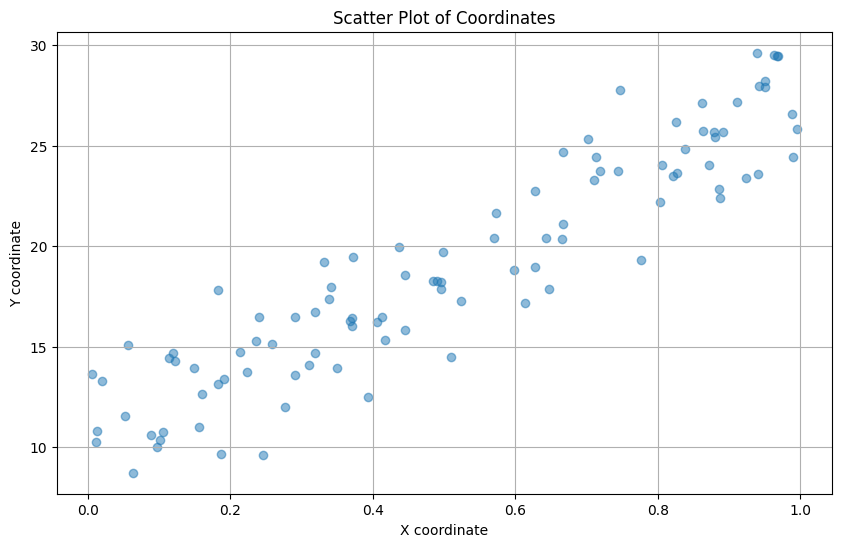
\includegraphics[width=0.5\textwidth]{images/4.1.png}
        \end{center}


	
     4.3 The shape of w should be a (1,2) (column) vector. This is because the points in the data are 2D.


    4.4 
    \begin{center}
        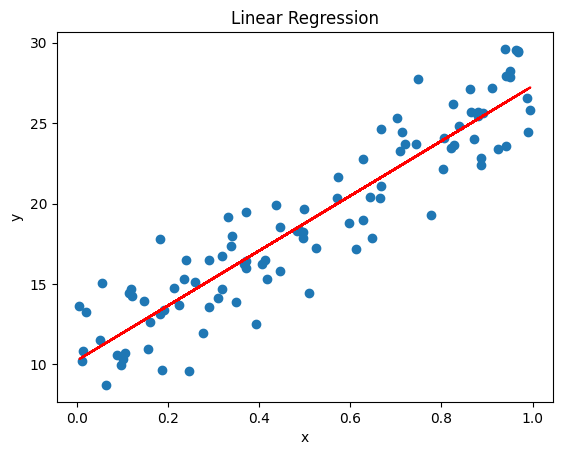
\includegraphics[width=0.5\textwidth]{images/4.4.png}
        \end{center}

        
\end{solution}

\end{document}